\documentclass[a4,paper,fleqn]{article}

\usepackage{../layout/layout}

\title{AE - FillCap - Messung 01}
\date{23. Oktober 2015}
\author{Yannick Inderbitzin\\
        Ervin Mazlagi\'c\\
        Yves Studer\\
        Daniel Winz}

\begin{document}
\maketitle
%\clearpage
\vfill
\tableofcontents
\vfill
\clearpage

\section{Sinn \& Zweck}
Die Messung des Füllstandes mittels kapazitivem Spannungsteiler soll getestet 
werden. 

\section{Messaufbau}
\begin{circuitikz}
    % Speiseschaltung
    \draw[]
        (1,2.5)
            to[short]
        (0,2.5)
            to[short]
        (0,0)
            to[V, l=$V_{in}$, v_=$40\si{\volt}_{pp}$]
        (6,0)
            to[short]
        (6,2.5)
            to[short]
        (5,2.5)
    ;
    % Messschaltung
    \draw[]
        (1.3,6.8)
            to[short]
        (2,6.8)
            to[short]
        (2,8)
            to[voltmeter, l=Oszilloskop]
        (4,8)
            to[short]
        (4,6.8)
            to[short]
        (4.7,6.8);
    ;
    % Primärer Kondensator
    \draw[] (1,2) -- (1,7) node[above] {$C_1$};
    \draw[] (5,2) -- (5,7) node[above] {$C_2$};
    % Sekundärer Kondensator
    \draw[] (1.3,2) -- (1.3,7);
    \draw[] (4.7,2) -- (4.7,7);
    \draw[latex-latex] (1.5,6) -- node[above] {$C_x$} (4.5,6);
    % Wasser
    \draw[thick, blue!50!, fill=blue!30!] (1.5,5) rectangle node[blue!80!] {$H_2O$} (4.5,2);
    \draw[ultra thick] (1.5,5.5) -- (1.5,2) -- (4.5,2) -- (4.5,5.5);
\end{circuitikz}

\section{Messmittel}
\begin{zebratabular}{llll}
    \rowcolor{gray}
    Messgerät       & Typ                   & Ser. Nr.      &Inv. Nr. \\
    Signalgenerator & Tektronix AFG 3252    & ????          & ???? \\
    Oszilloskop     & Agilent MSO6052A      & MY44008055    &117 \\
    LCR Meter       & GW Instek LCR-8110G   & ????          & - \\
\end{zebratabular}

\section{Ergebnisse}

\subsection{Amplitudenmessung bei verschiedenen Frequenzen}
\begin{minipage}{0.45\textwidth}
\begin{zebratabular}{llll}
    \rowcolor{gray}
    $f_{in}$ [\si{\hertz}] &
        $V_{e_{pp}}$ [\si{\volt}] &
        $V_{f_{pp}}$ [\si{\volt}] &
        $\Delta V$ [\si{\volt}] \\
    1k      & 3.206     & 3.137     & 0.069 \\
    10k     & 6.478     & 5.863     & 0.615 \\
    100k    & 6.341     & 5.662     & 0.679 \\
    200k    & 6.333     & 5.654     & 0.679 \\
    500k    & 6.310     & 5.638     & 0.672 \\
    1M      & 6.287     & 5.638     & 0.649 \\
    2M      & 6.213     & 5.580     & 0.633 \\
    5M      & 6.105     & 5.523     & 0.582 \\
    10M     & 9.723     & 8.500     & 1.223 \\
    20M     & 9.278     & 8.336     & 0.942 \\
    50M     & 17.08     & 15.26     & 1.82  \\
    100M    & 5.886     & 5.798     & 0.088 \\
\end{zebratabular}
\end{minipage}
\begin{minipage}{0.45\textwidth}
\begin{tikzpicture}
    \begin{semilogxaxis}[
        log basis x=10,
        grid=both,
        xmin=1e3,
        xmax=1e8,
        ymin=0,
        xlabel={$f$ [\si{\hertz}]}, 
        ylabel={$U$ [\si{\volt}]},
        ]
        \addplot file {mess01/amplitude_empty.table};
        \addlegendentry{empty}
        \addplot file {mess01/amplitude_full.table};
        \addlegendentry{full}

    \end{semilogxaxis}
\end{tikzpicture}
\begin{tikzpicture}
    \begin{semilogxaxis}[
        log basis x=10,
        grid=both,
        xmin=1e3,
        xmax=1e8,
        ymin=0,
        xlabel={$f$ [\si{\hertz}]}, 
        ylabel={$\Delta U$ [\si{\volt}]},
        ]
        \addplot file {mess01/amplitude_diff.table};

    \end{semilogxaxis}
\end{tikzpicture}
\end{minipage}

\subsection{Amplitudenspektrum}
\begin{minipage}{0.45\textwidth}
    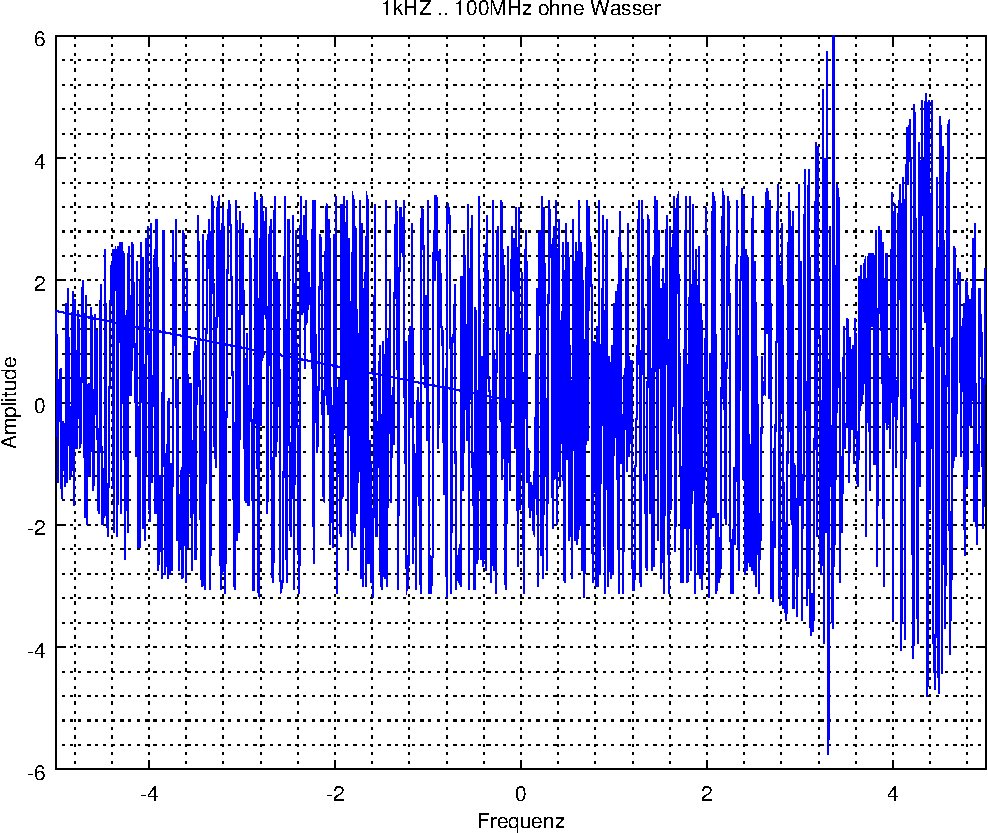
\includegraphics[width=1.0\textwidth]{mess01/scope_1.pdf}
    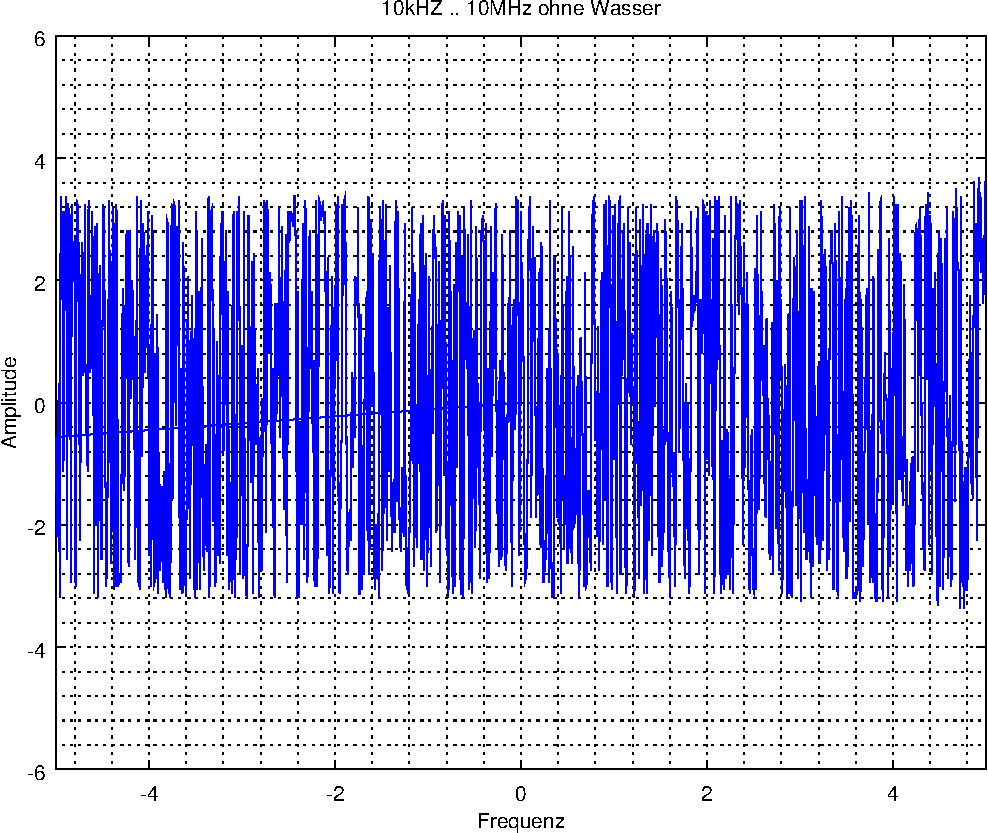
\includegraphics[width=1.0\textwidth]{mess01/scope_2.pdf}
\end{minipage}
\begin{minipage}{0.45\textwidth}
    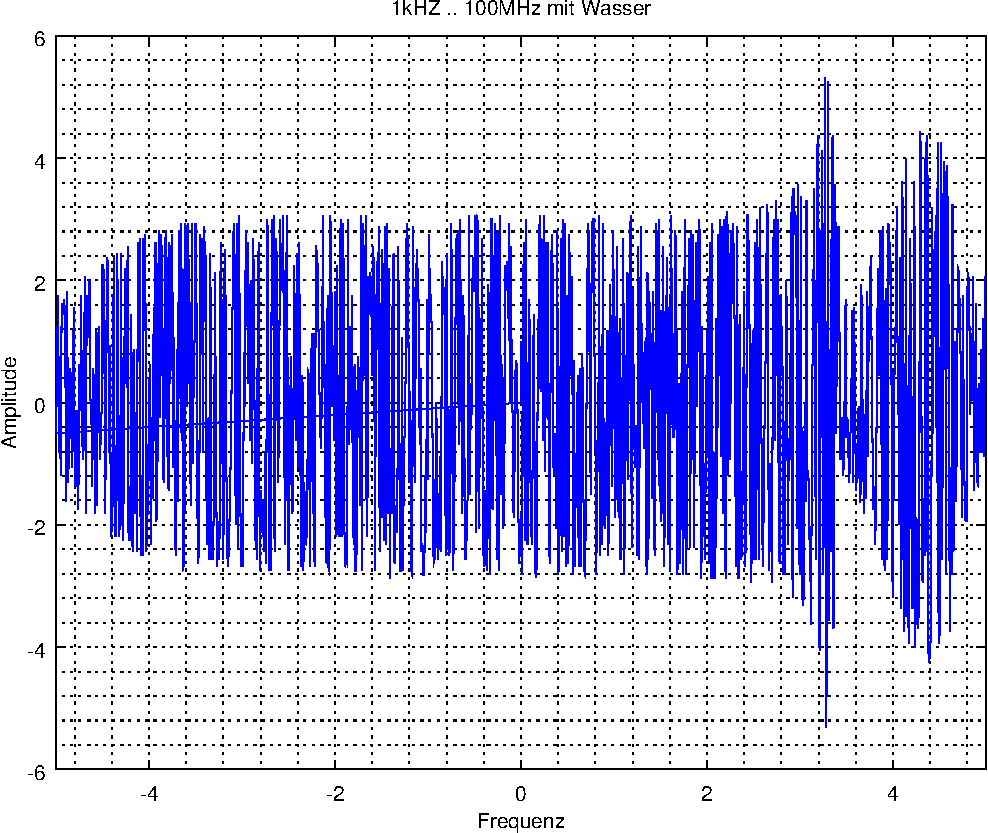
\includegraphics[width=1.0\textwidth]{mess01/scope_0.pdf}
    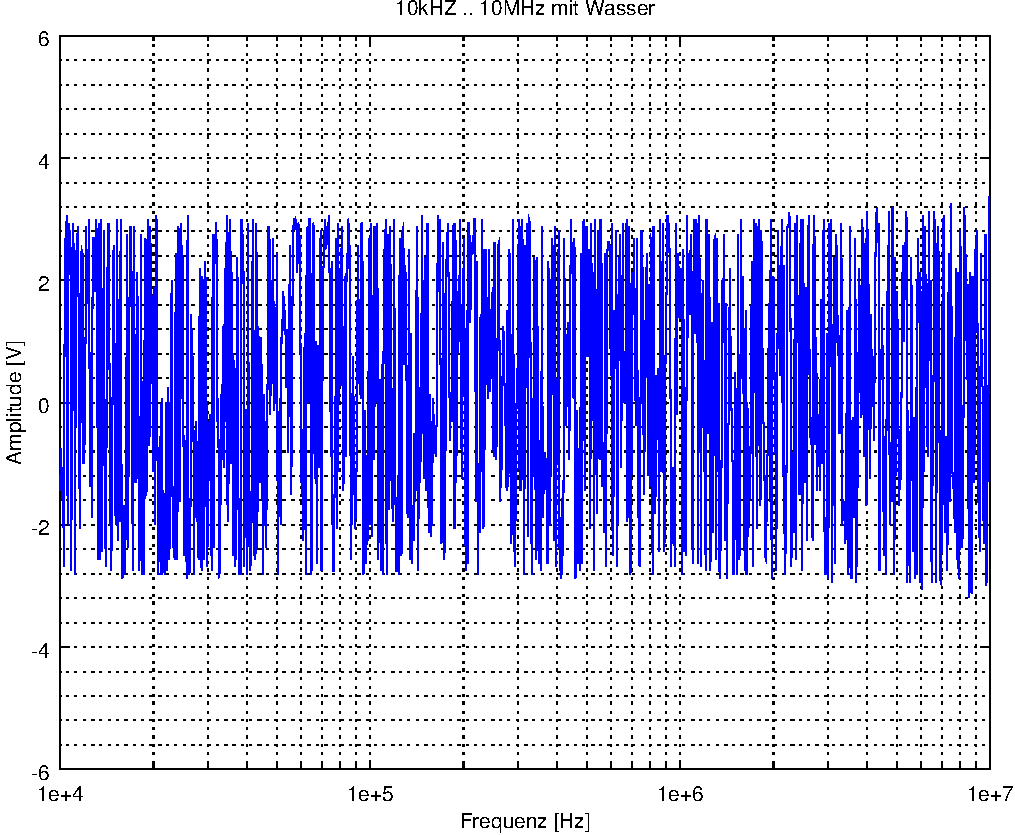
\includegraphics[width=1.0\textwidth]{mess01/scope_3.pdf}
\end{minipage}

\subsection{Kapazitätsmessung}
\begin{zebratabular}{lllll}
    \rowcolor{gray}
    $f_{in}$ [\si{\hertz}] &
        $C_{e_{pp}}$ [\si{\pico\farad}] &
        $Q_{e_{pp}}$ [1] &
        $C_{f_{pp}}$ [\si{\pico\farad}] &
        $Q_{f_{pp}}$ [1] \\
    100k    & 2.64  & 55    & 6.94  & 39 \\
    1M      & 2.61  & 86    & 6.73  & 26 \\
    10M     & 9.5   & 23    & 14.3  & 15 \\
\end{zebratabular}

\section{Fazit}
Die Änderung der Ausgangsspannung ist messbar. Somit kommt das Verfahren für 
die Messung des Wasserstandes in Frage. \\
Die Amplitude, als auch die Amplitudenänderung bleibt dabei im Bereich von 
10\si{\kilo\hertz} bis 5\si{\mega\hertz} konstant. \\
Auch die Kapazitätsänderung ist gut messbar. 

\end{document}
